
% This LaTeX was auto-generated from MATLAB code.
% To make changes, update the MATLAB code and republish this document.

\documentclass{article}
\usepackage{graphicx}
\usepackage{color}

\sloppy
\definecolor{lightgray}{gray}{0.5}
\setlength{\parindent}{0pt}

\begin{document}

    
    \begin{verbatim}
clear all;
clc;
p = @(x) -(x+1);
q = @(x) cos(x);
r = @(x) -exp(x);
a = 0;
b = 1;
h = 1/400;
alpha = 1;
beta = 3;
fprintf('Q1(a)\n');
fprintf('The plot for solution using Central difference for the first order derivative is\n');
central_diff(a,b,h,alpha,beta,p,q,r,1);
fprintf('The plot for solution using Backward difference for the first order derivative is\n');
backward_diff(a,b,h,alpha,beta,p,q,r,2);
fprintf('The plot for solution using Forward difference for the first order derivative is\n');
forward_diff(a,b,h,alpha,beta,p,q,r,3);
%(b)
p = @(x) -2;
q = @(x) -1;
r = @(x) -x;
a = 0;
b = 1;
h = 0.01;
alpha = 0;
beta = 0;
fprintf('Q1(b)\n');
fprintf('The plot for solution using Central difference for the first order derivative is\n');
central_diff(a,b,h,alpha,beta,p,q,r,4);
fprintf('The plot for solution using Backward difference for the first order derivative is\n');
backward_diff(a,b,h,alpha,beta,p,q,r,5);
fprintf('The plot for solution using Forward difference for the first order derivative is\n');
forward_diff(a,b,h,alpha,beta,p,q,r,6);

% functions

function y = central_diff(a,b,h,alpha,beta,p,q,r,fig_no)
t = [a:h:b];
n = length(t);
y = zeros(1,n);
y(1) = alpha;
y(n) = beta;

A = zeros(n-2,n-2);
b = zeros(n-2,1);
% i = 2
A(1,1) = (2/h^2 + q(t(2)));
A(1,2) = (-1/h + p(t(2))/2)/h;
b(1) = r(t(2)) - y(1)*(-1/h - p(t(1))/2)/h;
%i = n
A(n-2,n-3) = (-1/h - p(t(n-1))/2)/h;
A(n-2,n-2) = (2/h^2 + q(t(n-1)));
b(n-2) = r(t(n-1)) - y(n)*(-1/h + p(t(n-1))/2)/h;

for i=3:n-2
    A(i-1,i-2) =  (-1/h - p(t(i))/2)/h;
    A(i-1,i-1) = (2/h^2 + q(t(i)));
    A(i-1,i) = (-1/h + p(t(i))/2)/h;
    b(i-1) = r(t(i));
end
y(2:n-1) = A\b;
y(2:n-1) = A\b;
figure(fig_no);
plot(t,y);
xlabel('x');
ylabel('y(x)');
title('Central Difference');

end
function y = backward_diff(a,b,h,alpha,beta,p,q,r,fig_no)
t = [a:h:b];
n = length(t);
y = zeros(1,n);
y(1) = alpha;
y(n) = beta;

A = zeros(n-2,n-2);
b = zeros(n-2,1);
% i = 2
A(1,1) = (2/h^2 + p(t(2))/h + q(t(2)));
A(1,2) = -1/h^2;
b(1) = r(t(2)) - y(1)*(-1/h - p(t(1)))/h;
%i = n
A(n-2,n-3) = (-1/h - p(t(n-1)))/h;
A(n-2,n-2) = (2/h^2 + p(t(n-1))/h + q(t(n-1)));
b(n-2) = r(t(n-1)) - y(n)*(-1/h^2);

for i=3:n-2
    A(i-1,i-2) =  (-1/h - p(t(i)))/h;
    A(i-1,i-1) = (2/h^2 + p(t(i))/h + q(t(i)));
    A(i-1,i) = -1/h^2;
    b(i-1) = r(t(i));
end
y(2:n-1) = A\b;
y(2:n-1) = A\b;
figure(fig_no);
plot(t,y);
xlabel('x');
ylabel('y(x)');
title('Backward Difference');
end
function y = forward_diff(a,b,h,alpha,beta,p,q,r,fig_no)
t = [a:h:b];
n = length(t);
y = zeros(1,n);
y(1) = alpha;
y(n) = beta;

A = zeros(n-2,n-2);
b = zeros(n-2,1);
% i = 2
A(1,1) = (2/h^2 - p(t(2))/h + q(t(2)));
A(1,2) = (-1/h + p(t(2)))/h;
b(1) = r(t(2)) - y(1)*(-1/h^2);
%i = n
A(n-2,n-3) = -1/h^2;
A(n-2,n-2) = (2/h^2 - p(t(n-1))/h + q(t(n-1)));
b(n-2) = r(t(n-1)) - y(n)*(-1/h + p(t(n-1)))/h;

for i=3:n-2
    A(i-1,i-2) =  -1/h^2;
    A(i-1,i-1) = (2/h^2 - p(t(i))/h + q(t(i)));
    A(i-1,i) = (-1/h + p(t(i)))/h;
    b(i-1) = r(t(i));
end
y(2:n-1) = A\b;
figure(fig_no);
plot(t,y);
xlabel('x');
ylabel('y(x)');
title('Forward Difference');

end
\end{verbatim}

        \color{lightgray} \begin{verbatim}Q1(a)
The plot for solution using Central difference for the first order derivative is
The plot for solution using Backward difference for the first order derivative is
The plot for solution using Forward difference for the first order derivative is
Q1(b)
The plot for solution using Central difference for the first order derivative is
The plot for solution using Backward difference for the first order derivative is
The plot for solution using Forward difference for the first order derivative is
\end{verbatim} \color{black}
    
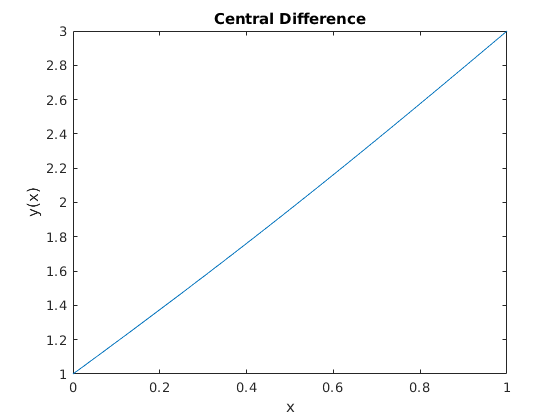
\includegraphics [width=4in]{lab9_q1_01.eps}

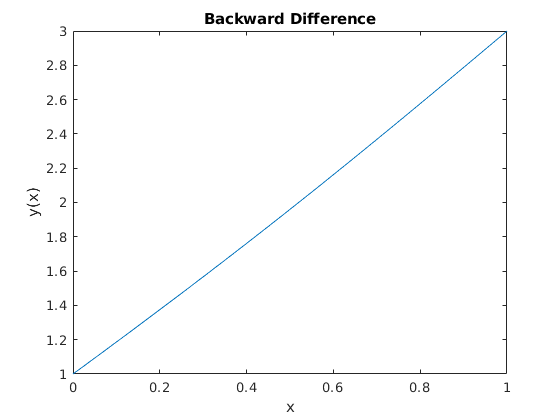
\includegraphics [width=4in]{lab9_q1_02.eps}

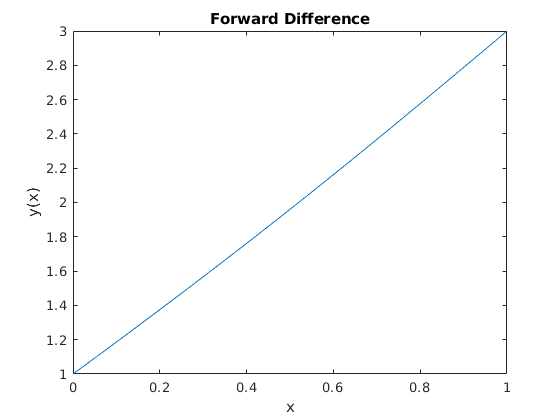
\includegraphics [width=4in]{lab9_q1_03.eps}

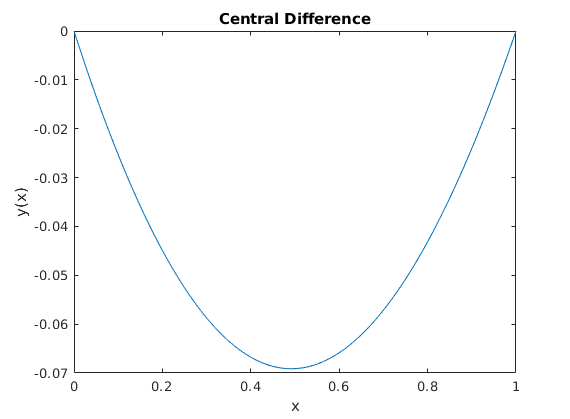
\includegraphics [width=4in]{lab9_q1_04.eps}

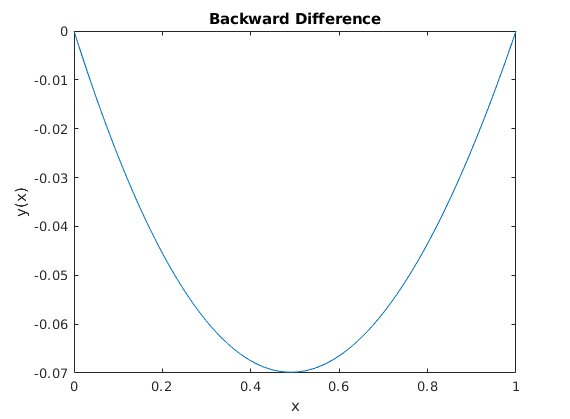
\includegraphics [width=4in]{lab9_q1_05.eps}

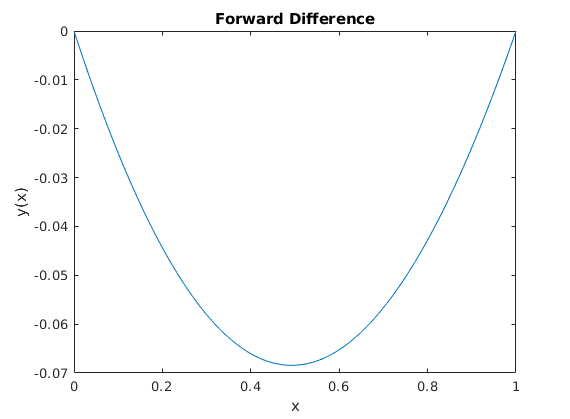
\includegraphics [width=4in]{lab9_q1_06.eps}



\end{document}
    
